	\newpage
\section{Ogólne określenie wymagań}		%1
%Ogólne określenie wymagań i zakresu programu (Czyli zleceniodawca określa wymagania programu) 















\subsection{Gra logiczna}  %1.1       

Projektem jest gra logiczna możliwa do zagrania tylko w trybie kooperacji. Gra będzie opierać się na stosunkowo łatwych zagadkach, które będzie można rozwiązać tylko współpracując.
\\Ogólnym konceptem jest podzielenie gry na 2 główne części:
\\\hspace{0.60cm}-Tryb graficzny,
\\\hspace{0.60cm}-Tryb tekstowy.


%
%rysunek

	\begin{figure}[!htb]
	\begin{center}
		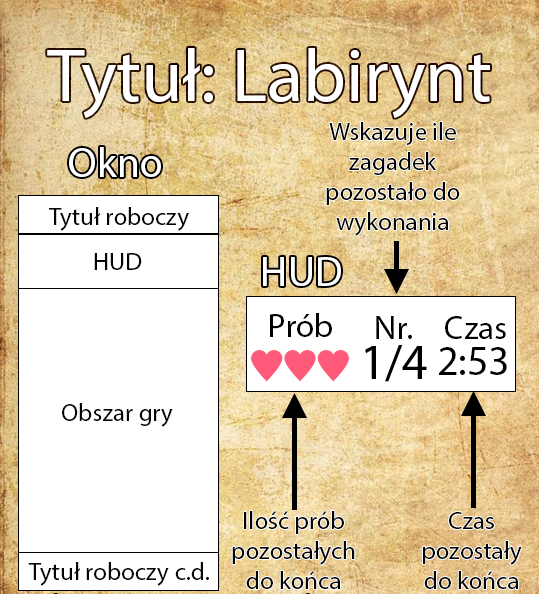
\includegraphics[width=8cm]{rys/gra1.png}
		\caption{Labirynt}
		\label{rys:rysunek001}
	\end{center}
\end{figure}

\hspace{-0.60cm}Jak możemy zauważyć na rysunku 1.1 będziemy mieli określoną liczbę żyć na rozwiązanie określonej liczby zagadek w określonym czasie. W tym trybie zagadki będą polegały na wyjściu z labiryntu.
\\
\\
\\
\\
\\
\\
\\
\\
	\begin{figure}[!htb]
	\begin{center}
		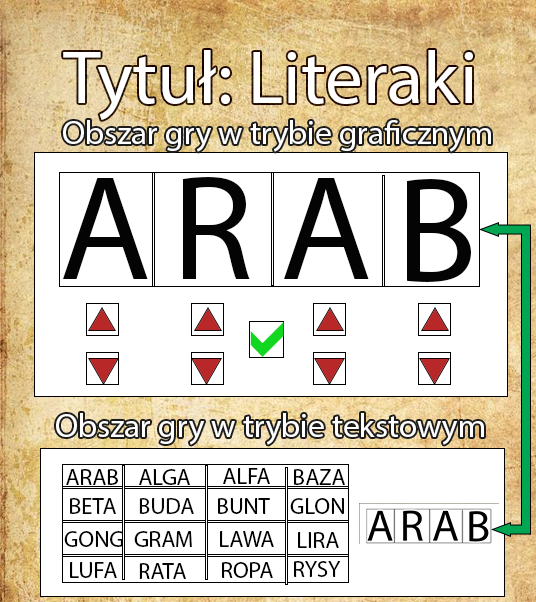
\includegraphics[width=8cm]{rys/gra4.png}
		\caption{Literaki}
		\label{rys:rysunek001}
	\end{center}
\end{figure}

\hspace{-0.60cm}W trybie gry Literaki gracze mają za zadanie ułożyć czteroliterowy wyraz, który nakłada się z wyrazem w bazie. Dostęp do bazy wyrazów ma gracz w trybie tekstowym. Gracz obsługujący tryb graficzny za pomocą strzałek zmienia litery na danej pozycji. 
\\Ze względu na to, ze nie wszystkie litery są na wszystkich polach możliwość będzie tylko jedna. Błędna kombinacja oznacza utratę jednego z żyć. Podobnie jak w trybie labiryntu po utracie 3 żyć gracze przegrywają.
\\
\\
\\
\\
\\
\\
\\
\\
\\
\\
\\
\\
\\
\\
	\begin{figure}[!htb]
	\begin{center}
		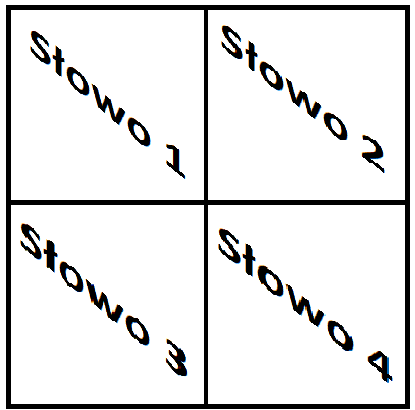
\includegraphics[width=8cm]{rys/gra5.png}
		\caption{Kod - Tryb graficzny}
		\label{rys:rysunek001}
	\end{center}
\end{figure}

	\begin{figure}[!htb]
	\begin{center}
		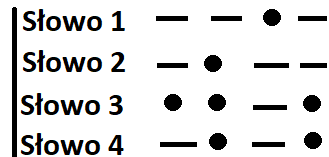
\includegraphics[width=8cm]{rys/gra6.png}
		\caption{Kod - Tryb tekstowy}
		\label{rys:rysunek001}
	\end{center}
\end{figure}
\hspace{-0.60cm}Trzeci tryb gry, który zostanie zaimplementowany do gry będzie oparty na latarce zawartej w telefonie. Telefon osoby obsługującej tryb graficzny włączy i wyłączy latarkę określoną liczbę razy tworząc przy tym "kod morsa" opisany w trybie tekstowym. Gracz obsługujący tryb graficzny będzie miał za zadanie zapamiętać stosunkowo krótki kod i podać go osobie będącej w trybie graficznym. Następnie osoba zarządzająca trybem graficznym musi dopasować go do jednego ze słów po czym podaje słowo kluczowe wspólnikowi. Wybór złego słowa pozbawia nas jednego życia i losuje nowy sygnał.
\\
\\
Kolejnym trybem gry będą "Kolorki". Będzie on polegał na odtworzeniu określonej sekwencji po jej wyświetleniu. Utrudnieniem będzie to, że każdy kolor będzie odpowiadał innemu, co będzie opisane w trybie graficznym. Gracz trybu graficznego będzie miał za zadanie komunikowania partnerowi jaki kolor został wyróżniony po czym kliknięcie w jego odpowiednik opisany w trybie tekstowym.
\\
\\
Ostatnia zagadka będzie stosunkowo prosta, będzie ona polegała na przytrzymaniu przycisku przez określony czas wtedy kiedy timer jako ostatnią cyfrę będzie miał cyfrę przypisaną do określonego koloru przycisku. Wszysko co musi wtkonać gracz w trybie graficznym jest opisane w trybie tekstowym.

\subsubsection{Tryb Graficzny}
Będzie opierał się na rozwiązywaniu zagadek. Gracz sam nie będzie w stanie rozwiązać zagadki, ponieważ podpowiedzi czy też cała solucja danej zagadki będą zawarte w trybie tekstowym.
W tym trybie będziemy widzieć plansze rozgrywki i będziemy mogli sterować naszą postacią.
\\
	\begin{figure}[!htb]
	\begin{center}
		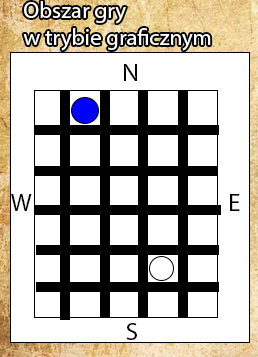
\includegraphics[width=8cm]{rys/gra2.png}
		\caption{Labirynt}
		\label{rys:rysunek001}
	\end{center}
\end{figure}

\hspace{-0.60cm}W trybie graficznym, jak widać na powyższym rysunku, widzimy naszą postać, niebieską kulkę, i nasz cel, białą kulkę. Natomiast nie widzimy drogi do mety~i w tym celu musimy komunikować się z partnerem.
\\
\\
Za każdym razem jak wykonamy zły ruch czyli wejdziemy w ścianę nasza kulka będzie wracać na początek trasy a my tracimy jedno z naszych żyć. Po utracie wszystkich żyć kończymy rozgrywkę.
\\
\\
Innym trybem gry będą literaki polegające na układaniu słów. Gracz w tym trybie będzie za pomocą strzałek zmieniał litery na określonych pozycjach. Błędna kombinacja prowadzi do utraty życia i jest równoznaczna z wejściem w ścianę w trybie labiryntu.
\\
\\
Tryb graficzny trzeciej gry będzie oparty na prostej tabeli z paroma różnymi opcjami do wyboru. W zależności od otrzymanych instrukcji od naszego wspólnika będziemy musieli wybrać jedną z nich. Telefon gracza obsługującego ten tryb będzie za pomocą latarki wyświetlał jeden z dwóch rodzajów sygnału. Bedzie to kod oparty o~kod morsa ale ze zmienionymi słowami. Dla przykładu jeżeli latarka włączy się raz na długo a potem 3 razy mrugnie będzie to oznaczało jeden sygnał długi (oznaczenie w trybie tekstowym - kreska) i 3 krótkie (w trybie tekstowym - kropka).
\\
\\
W trybie graficzny w czwartej zagadce będziemy musieli obserwować, który kolor zostaje wyróżniony. Następnie komunikujemy się z partnerem, który wskazuje nam odpowiadający kolor dla wyróżnionego po czym go klikamy. Sekwencja wydłuża się do pięciu wyróżnionych kolorów. Gra kończy się wraz ze zgadnięciem pięciu odpowiednich kolorów.
\\
\\
Ostatnia zagadka będzie stosunkowo prosta. Wymagane będzie od nas tylko przytrzymanie przycisku przez odpowiednio długi czas.
\subsubsection{Tryb Tekstowy}  %1.2

Będzie opierał się na znajdowaniu podpowiedzi czy też solucji do aktualnie wykonywanej zagadki przez osobę obsługującą tryb graficzny.
Naszym zadaniem będzie współpraca z osobą, która steruje postacią w trybie graficznym w celu jak najefektywniejszego ukończenia zagadek przed końcem ustalonego czasu.
\\
\\
\\
\begin{figure}[!htb]
	\begin{center}
		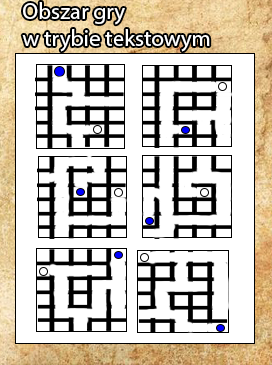
\includegraphics[width=8cm]{rys/gra3.png}
		\caption{Labirynt}
		\label{rys:rysunek001}
	\end{center}
\end{figure}

\hspace{-0.60cm}Jak można zobaczyć na rysunku 1.6 w trybie tekstowym będziemy widzieć dostępne mapy rozgrywki. Zadaniem gracza w trybie teksowym będzie takie poprowadzenie partnera w trybie graficznym, żeby niebieska kula dotarła do~mety (białej kuli) unikając wchodzenia w ściany. 
\\
\\
W trybie gry "Literaki"~gracz (obsługujący tryb tekstowy) będzie miał dostępną bazę ze słowami i będzie musiał dzięki komunikacji z graczem operującym interfejsem graficzym pomóc mu ułożyć pasujące słowo. Gracz w trybie graficznym będzie miał opcję ułożenia tylko jednego słowa z bazy.
 \\
 \\
 W trzecim trybie gry będziemy musieli za pomocą komunikacji z naszym partnerem rozszyfrować o jaki kod chodzi w danym momencie. W trybie tekstowym będziemy otrzymywać informacje dotyczące "wyglądu kodu". W rzeczywistości ostrzymamy informację ile było długich sygnałów a ile krótkich i w jakiej kolejności. Po otrzymaniu takowych informacji gracz będzie stawał przed wyborem jednego ze słów, które w tym przypadku będzie oznaczone przed chwilą otrzymanym kodem. Jeżeli żadne słowo się nie będzie zgadzać to najprawdopodobniej otrzymaliśmy złe podpowiedzi od naszego partnera. Jeżeli jednak znajdujemy pasujący kod to podajemy słowo, które ten kod opisuje do operatora trybu graficznego. 
 \\
 \\
 W czwartej zagadce będziemy mieli opisane, który kolor odpowiada któremu. Dla przykładu jeżeli zostanie wyróżniony kolor zielony to naszym zadaniem będzie poszukanie, który kolor jest przypisany do niego (na przykład czerwony) i zakomunikowanie tego naszemu partnerowi.
 \\
 \\
 W piątej zagadce będziemy mieli opis jaki kolor przycisku odpowiada ilości przytrzymanych sekund i jaka musi być ostatnia cyfra na timerze. Po sprawdzeniu tego przekazujemy naszemu partnerowi wszyskie te informacje a on kończy w ten sposób grę.
 
 
 